\chapter{Likelihoods and cosmological parameters}\label{ch:likelihoods_cosmology}
 
Bayes theorem\index{Bayes theorem}

What we are interested in is an understanding of the probability for a particular model to represent the universe, given the data that we have measured.  We can schematically write this as $P(\mbox{model}|\mbox{data})$.

In the context of supernova cosmology measuring the background expansion of a $\Lambda$CDM universe model, what we are really constraining is some set of parameters $\Theta$, where in this case we might have the particular cosmological parameters
\begin{equation}
  \Theta = (\Omega_m,\Omega_\Lambda,\Omega_k, H_0),
\end{equation}
while later we will add additional cosmological parameters about the baryon density, initial fluctuations, reionization, neutrinos, and more once  we include further data that can constrain them.

The specific data vector is measurements of the distance modulus--redshift relationship for a set of supernovae
\begin{equation}
  d = \{  (\mu_i,z_i) \mbox{ for SN }i \},
\end{equation}
but we could have swapped luminosity distances for distance moduli.  Later we will include or swap in other types of data in one gigantic vector.  
We also have to have a notion of our uncertainty about this data.  If we consider $d = s+ n$, we need to know the covariance $C_{\rm SN}$ of the noise part.  For supernova, 
we have the contribution from the measurement uncertainty of the photometry of each individual, independent supernova, but we also have the modeling uncertainty from the spectral model (SALT2), which is correlated across all supernovae.  The redshifts are usually measured with such precision through spectroscopy that their uncertainties are negligable, but in other circumstances (SN with only photometric redshift estimates) you would need to include those as well.

Thus we are looking for the probability density
\begin{equation}
  p(\Theta| d)
\end{equation}
which we can integrate up to learn what the probability is for the cosmological parameters to be in any particular volume in parameter space
\begin{equation}
  P( \Theta \in \Delta \Theta | d ) = \int_{\Delta\Theta} d\Theta\  p(\Theta| d)
\end{equation}
Although this probability of model given data is hard to compute, there is a key result in probability, called Bayes theorem, that allows us to cast it as something that is easy for us to compute.

\section{Bayes theorem}
Both the data and the parameters they lead to are random variables, so we need to understand how to deal with the probability that one event is true (the model) given another event is true (the data we measured).

\begin{figure}
  \begin{center}
    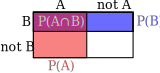
\includegraphics[width=0.7\textwidth]{figs/cosmological_parameters/bayes_theorem.pdf}
  \end{center}
  \caption{Diagram for Bayes theorem.  The probability for event A is in red and the probability for event B is in blue.  These overlap to form purple in the region of the probability of both events occurring jointly.} \label{fig:bayes_theorem}
\end{figure}

Let's step away for a moment and examine a truth table for two generic events, $A$ and $B$, as in Figure \ref{fig:bayes_theorem}.  We have probability $P(A)$ that $A$ has occurred, and $1-P(A)$ is the probability that not-$A$ has occurred.  Between $A$, not-$A$, $B$, and not-$B$, we have covered all the possibilities.  The probability that both $A$ and $B$ occurred jointly is $P(A \cap B)$, which is only a fraction of the total probability for $P(B)$.

So if we know that $B$ has occurred, then the probability that A also will occur is just that fraction:
\begin{equation}
  P(A|B) = \frac{P(A\cap B)}{P(B)},
\end{equation}
which defines precisely what we mean by the conditional probability of $A$ given that $B$ occurred.
On the other if we knew $A$ occurred, then the fractional probability of $B$ is similarly
\begin{equation}
  P(B|A) = \frac{P(A\cap B)}{P(A)}.
\end{equation}

Multiplying through by the denominators we find the relation between the conditional probabilities      
\begin{equation}
  P(A|B) P(B) = P(A \cap B) =   P(B|A) P(A).
\end{equation}
This results is called Bayes theorem\index{Bayes theorem}.
What about probability densities?  Well, the probabilities are the integrals of the density and joint density
\begin{equation}
  P(A)  = \int_{\Delta A} da\  p(a)\qquad \mbox{and} \qquad  P(A \cap B)  = \int_{\Delta A}\int_{\Delta B} da\  p(a,b)
\end{equation}
and so
\begin{equation}
 \int_{\Delta B} \int_{\Delta A} p(a|b) p(b) =  \int_{\Delta A} \int_{\Delta B} p(b|a) p(a)
\end{equation}
This is true regardless of the integration interval, so that means the integrands themselves must be equal:
\begin{equation}
  p(a|b) p(b) =  p(b|a) p(a)
\end{equation}

Now let's step back to the context of science.  Substituting in the model and data, and rearranging, the quantity that we are targeting---the \textit{posterior probability}\index{posterior probability} $p(\Theta | d )$---has the following expression:
\begin{equation}
  p(\Theta | d ) = \frac{1}{p(d)} p(d | \Theta) p(\Theta) \label{eqn:bayes_density}
\end{equation}
It is called the posterior probability because it is the probability that we find after taking our data.  The other pieces have names. The \textit{prior probability}\index{prior probability} $p(\Theta)$ are the chances that we assigned to some parameter values before we got our data.  The prior probability can come through a theoretical understanding (e.g. we don't expect matter density to be negative) or from previous measurements that we are taking as well-established.  In the simplest case we can use a flat prior\index{flat prior} with a uniform probability distribution.

The \textit{likelihood}\index{likelihood} $p(d | \Theta)$ is the probability that our dataset came from a particular cosmological model parameterized by $\Theta$, even if it's not the right one.  If we understand the predictions of our model and the uncertainties of our measurement, that is something we can usually compute.  Because it is so important, the likelihood is sometimes given its own symbol ${\cal L}(d|\Theta)$.

Perhaps surprisingly, the normalization factor, $1/p(d)$, the probability of our data, is not very important.  This is because the methods we use to evaluate the posterior only require a function that is proportional to the posterior.  Besides that, the posterior (Equation \ref{eqn:bayes_density}) is a probability distribution, and should integrate to unity over all parameters, so we can normalize it after the fact.

%\section{Gaussian likelihood in the case of supernovae}

We can easily build a Gaussian likelihood for the supernova data given the ingredients on hand:
\begin{equation}
  {\cal L}(\Theta|d) =  \frac{1}{(2\pi |C_{\rm SN}|)^{n/2}} \exp( - \chi_{\rm SN}^2/2 )
\end{equation}
where
\begin{equation}
\chi^2_{\rm SN} = (\mu - \mu^{th}(z| \Theta  ))^\dag C_{\rm SN}^{-1} (\mu - \mu^{th}(z| \Theta  ))  ).
\end{equation}
This is easy to compute.
Once again, in this case, the normalization of the likelihood is not important.
  
\section{Markov Chain Monte Carlo}

We can now evaluate the posterior probability for any model that we want, in principle, by drawing a grid in our parameter space and evaluating the likelihood times any prior at each grid point.  Unfortunately, this method suffers from the ``curse of dimensionality'' when we have a large number of parameters.  If it takes a hundred points to draw a nice smooth curve for the posterior, we have to evaluate $100^{N_{\rm par}}$ points to complete the grid.  Furthermore, we are not always sure where the peak of the posterior is, and its contours could be thin and not well-aligned with our parameter grid.  We could miss the details.

\begin{figure}
  \begin{center}
    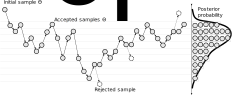
\includegraphics[width=\textwidth]{figs/cosmological_parameters/mcmc.pdf}
  \end{center}
  \caption{The Markov Chain Monte Carlo procedure for estimating a posterior probability distribution. In this schematic example, about ninety percent of the samples are accepted, which would be unacceptably high in a real application. {Figure adapted from \citet{en8065538}.}} \label{fig:MCMC}
  \end{figure}

The Markov Chain Monte Carlo (MCMC)\index{Markov Chain Monte Carlo} method helps us to sample the parameter space in a more efficient way.  A Markov chain or Markov process is stochastic chain of points in parameter space where the next step depends only on the current step.  In an MCMC chain, we set up a process so that the points $\Theta_i$ contained in the chain have the same distribution as the posteriors probability.  That is, the points are samples of the posterior distribution.  Figure \ref{fig:MCMC} illustrates how a histogram built from the samples of the chain can approximate the posterior probability.
For a multidimensional parameter space, the marginal distributions of the individual parameters are simply the one-dimensional histograms of that parameter's value in the points of the chain.

Furthermore, we can use the sample of the chain to evaluate any integral over the posterior.  For example, to compute the mean of parameter $\Theta_a$ we can approximate the integral as a sum over the points in the chain:
\begin{equation}
  \langle \Theta_a \rangle = \int d\Theta\  \Theta_a\  p(\Theta | d) \approx \frac{1}{N_{\rm chain}}\sum_i \Theta_{a,i} 
\end{equation}

So next we will look at the condition needed to set up such a Markov process and two algorithms for carrying it out.

\subsubsection{Detailed Balance}
We can imagine that the point in our chain are like the quantum mechanical hops of a particle in a potential well.  The principle of detailed balance in thermodynamics states that at equilibrium the every process is in equilibrium with the reverse process.  We want the distribution of points to be achieve an equilibrium, stationary distribution that matches our desired distribution.  We will have a transition probability to hop from state $\Theta$ to state $\Theta'$.  Detailed balance tells us that the probability of being in state $\Theta$ times the probability of jumping from there to $\Theta'$ is the same as the reverse, being in state $\Theta'$ times the probability of jumping to $\Theta$.  In equations, that condition is:
\begin{equation}
  p(\Theta'|\Theta) p(\Theta|d) =   p(\Theta|\Theta') p(\Theta'|d) 
\end{equation}
which gives us the condition on the transition probability
\begin{equation}
  \frac{p(\Theta'|\Theta)}{  p(\Theta|\Theta')}  =  \frac{p(\Theta'|d) }{p(\Theta|d)}.
\end{equation}

\subsubsection{Metropolis-Hastings algorithm}
The Metropolis-Hastings algorithm breaks the hop into two steps.  First, there is a proposed next state.  Second, this proposal with some probability is accepted (make the jump)  or rejected (stay at the location for one more turn), in which case the next state is set to be the same as the current state.  Let's explore how this can satisfy the detailed balance condition.

We write the transition probability as 
\begin{equation}
  p(\Theta'|\Theta) = g(\Theta'|\Theta) A(\Theta'|\Theta)
\end{equation}
where $g(\Theta'|\Theta)$ is the proposal probability and $A(\Theta'|\Theta)$ is the acceptance probability.

Thus detailed balance is satified when
\begin{equation}
  \frac{A(\Theta'|\Theta)} { A(\Theta|\Theta')} =  \frac{p(\Theta'|d) }{p(\Theta|d)} \frac{g(\Theta|\Theta')}{g(\Theta'|\Theta)} \label{eqn:acceptance_detailed_balance_condition}
\end{equation}

A choice that does this is
\begin{equation}
  A(\Theta'|\Theta) = {\rm  min} \left( 1,   \frac{p(\Theta'|d) }{p(\Theta|d)} \frac{g(\Theta|\Theta')}{g(\Theta'|\Theta)}  \right). \label{eqn:MH_acceptance}
\end{equation}
The value of the minimum function depends on whether the numerator or the denominator of the fraction is larger.  In either case, we satisfy the condition of detailed balance \ref{eqn:acceptance_detailed_balance_condition}.  Often we will use a symmetric proposal distribution, for example, a gaussian-normal distribution
\begin{equation}
  g(\Theta'|\Theta) = \frac{1}{(2\pi |C_{\rm prop}|)} \exp (-(\Theta'- \Theta)^\dag C^{-1}_{\rm prop}(\Theta'- \Theta)/2). \end{equation}
A symmetric proposal cancels in Equations \ref{eqn:acceptance_detailed_balance_condition} and \ref{eqn:MH_acceptance}, simplifying the detailed balance condition.  For a symmetric distribution, jumps into higher probability regions of parameter space are always accepted.

\paragraph{MCMC Metropolis Hastings recipe.}   Here a illustrate a typical parameter pipeline, which looks like this:
\begin{enumerate}
\item Initialize parameters with values $\Theta_0$ and compute the posterior probability of that point $p(\Theta_0|d)$.
  
\item Loop over the samples in the chain $\Theta_i$:
  \begin{enumerate}
  \item Propose a new sample $\Theta' ~ {\cal N}(\Theta_i,C_{\rm prop})$ (for a symmetric gaussian-normal, or use some other distribution $g$).
    \item Compute the posterior probability $p(\Theta'|d)$
  \item Compute the acceptance probability $$ A = {\rm  min} \left( 1,   \frac{p(\Theta'|d) }{p(\Theta|d)} \frac{g(\Theta|\Theta')}{g(\Theta'|\Theta)}  \right).$$
  \item Generate a uniform random deviate $u \sim U(0,1)$.
    \begin{enumerate}
    \item If $u \leq A$, accept the sample and set $\Theta_{i+1} = \Theta'$.
    \item If $u > A$, reject the sample and set $\Theta_{i+1} = \Theta_i$, repeating the previous sample.
    \end{enumerate}
  \end{enumerate}
\item Discard the initial samples, taking only those after the chain has time to ``burn in.''
\item Examine the autocorrelation length, convergence, and acceptance probabilities of the chain.  Several chains can be run in parallel and compared.
\item Use the samples to approximate the posterior: compute means/medians, confidence intervals, and statistics of the parameters.
\end{enumerate}

You want to tune your proposal distribution so that it explores the probability distribution.  If the acceptance probability is too high (averaging above 0.5), it can indicated that the typical step size is too small, and your chain is not departing the high-probability region and will explore the distribution very slowly.  We will talk about correlations in the next chapter, but small steps leads to a long autocorrelation length, meaning that the effective number of independent samples is much smaller than the total number of samples.

Similarly, if the acceptance probability is too low (averaging below 0.1), the proposed jumps are likely too large and are landing is regions of such low probability the jump is rarely made.  The samples stay put for long periods of time, leading to slow exploration.

For high-dimensional ($N_{\rm par} > 5$) problems, the optimal acceptance rate is about $\langle A \rangle = 0.2$--$0.25$.  For low-dimensional problems, optimal acceptance is higher $\langle A \rangle = 0.4$--$0.5$.

The initial point of the chain may not be close to the high-probability portion of the parameter space.  It is necessary to allow the chain to ``burn in'' before it can be usefully employed: to explore, find the high probability region, and get settled there.  The initial part of the chain should thus be discarded.

multimoded distributions are particularly difficult.

Fuzzy caterpillar versus wiggly snake.

Gelman-Rubin statistic


\subsubsection{Affine invariant algorithm}


emcee \citep{2013PASP..125..306F}





\subsubsection{Gibbs sampling}
Or maybe delay this to the CMB chapter

\subsubsection{Model selection}

Bayesian evidence

Model selection

``Suspiciousness'' and ``Index of Inconsistency'' which I don't know what they are.

\subsubsection{Confidence intervals}
credible intervals



\section{Simulation-based inference}



\section*{Exercises}
\begin{enumerate}

\item Check both cases, that the numerator or the denominator is larger, to show that Equation~\ref{eqn:MH_acceptance} satifies the condition of detailed balance.

  \end{enumerate}
